\documentclass{article}

\usepackage{amsmath}
\usepackage{amssymb}
\usepackage{amsthm}
\usepackage{tikz}
\usetikzlibrary{automata, positioning, arrows.meta}

\theoremstyle{definition}
\newtheorem{definition}{Definition}
\newcommand{\tuple}[1]{\langle #1 \rangle}

\begin{document}

\section{State-Quantified Hyperautomata}

\subsection{Intuition}
Standard Finite-Word Hyperautomata (NFH) operate on a static assignment of words to variables, determined entirely before the run begins. This limits the automaton to verifying properties where the witness words are pre-selected. We introduce the \textit{State-Quantified NFH} (SQ-NFH) to allow for \textit{dynamic variable extension}. In this model, the automaton can query the input hyperword $S$ during execution to append new words to its variables. This capability is formalized by a labeling function $L$ that enforces extensions: if a state is labeled with a variable index, the machine must pick a word from $S$ and append it to that variable's buffer before processing any transitions. The rest of the definitions are as defined in regular NFH.

\subsection{Formal Definition}

\begin{definition}[Configuration]
Let $\Sigma$ be a finite alphabet. A configuration is a tuple $c = (q, u_1, \dots, u_k)$, where $q$ is a state and $u_i \in \Sigma^*$ represents the current content of the buffer for variable $x_i$. For a step $j$ in a run, we denote the \textit{ingress configuration} as $c_j^{in}$ and the \textit{egress configuration} as $c_j^{out}$.
\end{definition}

\begin{definition}[SQ-NFH]
A State-Quantified Non-deterministic Finite Hyperautomaton is a tuple $\mathcal{A} = \tuple{\Sigma,X,Q,Q_0,F,\delta,\alpha,L}$, where:
\begin{itemize}
    \item $\Sigma$ is the finite alphabet.
    \item $X = \{x_1, \dots, x_k\}$ is a finite set of word variables.
    \item $Q$ is a finite set of states.
    \item $Q_0 \subseteq Q$ is the set of initial states.
    \item $\delta \subseteq Q \times (\Sigma \cup \{\#\})^{k} \times Q$ is the transition relation.
    \item $F \subseteq Q$ is the set of accepting states.
    \item $\alpha = Q_1 x_1 Q_2 x_2 \dots Q_k x_k$ is a quantifier prefix, where $Q_i \in \{\forall, \exists\}$ for every $1 \leq i \leq k$.
    \item $L \subseteq Q \times \{1, \dots, k\}$ is the extension labeling relation. If $(q, i) \in L$, variable $x_i$ must be extended at state $q$.
\end{itemize}
\end{definition}

\noindent \textbf{Semantics.} The semantics of an SQ-NFH are defined with respect to a hyperword $S$. Let $v: X \to S$ be an assignment of the word variables of $\mathcal{A}$ to words in $S$. We denote by $v[x \to w]$ the assignment obtained from $v$ by assigning the word $w \in S$ to $x \in X$. We denote the satisfaction relation as $S \models_v (\alpha, \mathcal{A})$, where $\alpha$ is a quantifier prefix, and define it as follows.
\newpage

\begin{enumerate}
    \item If $\alpha = \exists x_i \beta$, then $S \models_v (\alpha, \mathcal{A})$ iff there exists $w \in S$ such that $S \models_{v[x_i \mapsto w]} (\beta, \mathcal{A})$.
    \item If $\alpha = \forall x_i \beta$, then $S \models_v (\alpha, \mathcal{A})$ iff for all $w \in S$, $S \models_{v[x_i \mapsto w]} (\beta, \mathcal{A})$.
    \item If $\alpha = \epsilon$, then $S \models_v (\epsilon, \mathcal{A})$ iff there exists a sequence of configuration pairs $\rho = (c_0^{in}, c_0^{out}), \dots, (c_m^{in}, c_m^{out})$ satisfying:
    \begin{itemize}
        \item \textbf{Initialization:} $c_0^{in} = (q_0, v(x_1), \dots, v(x_k))$ for some $q_0 \in Q_0$.
        \item \textbf{Quantification:} For every $0 \le j \le m$, let $c_j^{in} = (q_j, u_1, \dots, u_k)$. The egress configuration $c_j^{out} = (q_j, u'_1, \dots, u'_k)$ satisfies:
        \begin{itemize}
            \item If $(q_j, i) \in L$, then $u'_i = u_i \cdot w$ for some $w \in S$.
            \item If $(q_j, i) \notin L$, then $u'_i = u_i$.
        \end{itemize}
        \item \textbf{Transition:} For every $0 \le j < m$, let $c_j^{out} = (q_j, u'_1, \dots, u'_k)$ and $c_{j+1}^{in} = (q_{j+1}, u''_1, \dots, u''_k)$. There exists a transition vector $\vec{\sigma} = (\sigma_1, \dots, \sigma_k) \in (\Sigma \cup \{\#\})^k$ such that $(q_j, \vec{\sigma}, q_{j+1}) \in \delta$ and for all $i$:
        \begin{itemize}
            \item If $\sigma_i \in \Sigma$, then $u'_i = \sigma_i \cdot u''_i$.
            \item If $\sigma_i = \#$, then $u'_i = u''_i$ (Asynchronous).
        \end{itemize}
        \item \textbf{Acceptance:} $c_m^{out} = (q_m, \epsilon, \dots, \epsilon)$ with $q_m \in F$.
    \end{itemize}
\end{enumerate}

\noindent \textbf{Note.} When discussing an SQ-NFH accepting a hyperword, the quantifier prefix $\alpha$ covers all variables in the automaton. Therefore, we can write $S \models \mathcal{A}$ without specifying an explicit assignment $v$.

\begin{definition}[Hyperlanguage of SQ-NFH]
The hyperlanguage recognized by an SQ-NFH $\mathcal{A}$ with quantifier prefix $\alpha$, denoted $\mathcal{L}(\mathcal{A})$, is the set of hyperlanguages $S$ that satisfy the automaton:
\[
\mathcal{L}(\mathcal{A}) = \{ S \subseteq \Sigma^* \mid S \models \mathcal{A} \}
\]
\end{definition}

\newpage

% \section{Expressiveness: The Composite Word Example}

% To demonstrate that State-Quantified Hyperautomata (SQ-NFH) are strictly more expressive than standard Finite-Word Hyperautomata (NFH), we present a hyperlanguage that requires dynamic variable extension to be verified.

% \subsection{The Hyperlanguage $H_{composite}$}

% Let $\Sigma = \{a\}$. We define the hyperlanguage $H_{composite}$ as the set of all sets $S \subseteq \Sigma^*$ that contain a ``composite word'': a word $w \in S$ that can be formed by concatenating two or more other words from $S$. Formally:
% \[
% S \in H_{composite} \iff \exists w, u_1, u_2, \dots, u_m \in S \text{ such that } m \ge 2 \text{ and } w = u_1 \cdot u_2 \cdots u_m
% \]

% \subsection{Inadequacy of Regular NFH}
% A standard NFH is defined with a fixed number of variables, $k$. To accept $H_{composite}$, the automaton must witness the decomposition of $w$ into its constituent parts $u_i$. 

% Consider the set $S_k = \{ a, a^{k+1} \}$. The only valid composite relation in $S_k$ is $a^{k+1} = \underbrace{a \cdot a \cdots a}_{k+1 \text{ times}}$. To verify this, an automaton requires $k+2$ logical ``slots'': one for the target word $a^{k+1}$ and $k+1$ for the instances of $a$. An NFH with only $k$ variables cannot simultaneously track all necessary components of this relation. Since $k$ is fixed for the automaton but the required decomposition length can be arbitrarily large, no single NFH can accept $H_{composite}$.

% \subsection{SQ-NFH Construction}
% The SQ-NFH can accept $H_{composite}$ using only two variables by dynamically extending the second variable to match the parts against the target.

% \begin{definition}[Automaton for $H_{composite}$]
% Let $\mathcal{A} = \langle \Sigma, \{x_1, x_2\}, Q, q_{start}, F, \delta, \exists x_1 \exists x_2, L \rangle$, where:
% \begin{itemize}
%     \item $Q = \{ q_{start}, q_{match}, q_{next}, q_{acc} \}$.
%     \item $F = \{ q_{acc} \}$.
%     \item $L = \{ (q_{next}, 2) \}$. This label forces the extension of variable $x_2$ whenever the state $q_{next}$ is reached.
%     \item $\delta$ is defined to simulate the concatenation check:
%     \begin{enumerate}
%         \item \textbf{Initialization:} 
%         \[ (q_{start}, \epsilon, q_{match}) \]
%         Transition silently to the matching phase.
        
%         \item \textbf{Match Characters:} 
%         \[ (q_{match}, (\sigma, \sigma), q_{match}) \quad \forall \sigma \in \Sigma \]
%         Verify that the character in the target $x_1$ matches the character in the current part $x_2$.
        
%         \item \textbf{Part Finished (Refill):} 
%         \[ (q_{match}, (\sigma, \#), q_{next}) \quad \forall \sigma \in \Sigma \]
%         If variable $x_2$ becomes empty (reads $\#$) but $x_1$ still has data ($\sigma$), transition to $q_{next}$ to trigger an extension.
        
%         \item \textbf{Extension Loop:} 
%         \[ (q_{next}, (\sigma, \sigma), q_{match}) \quad \forall \sigma \in \Sigma \]
%         At $q_{next}$, the label in $L$ forces $x_2$ to be extended with a new word from $S$. We immediately compare the first character of this new word against the character $\sigma$ from $x_1$ that was pending.
        
%         \item \textbf{Acceptance:} 
%         \[ (q_{match}, (\#, \#), q_{acc}) \]
%         If both $x_1$ and $x_2$ become empty simultaneously, the concatenation is valid.
%     \end{enumerate}
% \end{itemize}
% \end{definition}

% This automaton effectively verifies $x_1 = x_2 \cdot x_2' \cdot x_2'' \dots$ for an arbitrary number of extensions, proving that SQ-NFH can capture properties defined by unbounded concatenations.



\section{SQ-NFH for $H_{chain}^{\$}$}

\subsection{Formal Definition}
\begin{definition}[Automaton for $H_{chain}^{\$}$]
Let $\Sigma = \{0, 1, \dots, n, \$\}$. We define the SQ-NFH $\mathcal{A} = \langle \Sigma, X, Q, q_0, F, \delta, \alpha, L \rangle$ as follows:
\begin{itemize}
    \item $X = \{x_1, x_2\}$, $\alpha = \exists x_1 \forall x_2$, $F = \{q_{acc}\}$.
    \item $L = \{ (q, 1) \mid q \in Q_{ext} \}$.
    \item $\delta$ is defined visually below.
\end{itemize}
\end{definition}

\subsection{Automaton Diagram}

\begin{figure}[h]
    \centering
    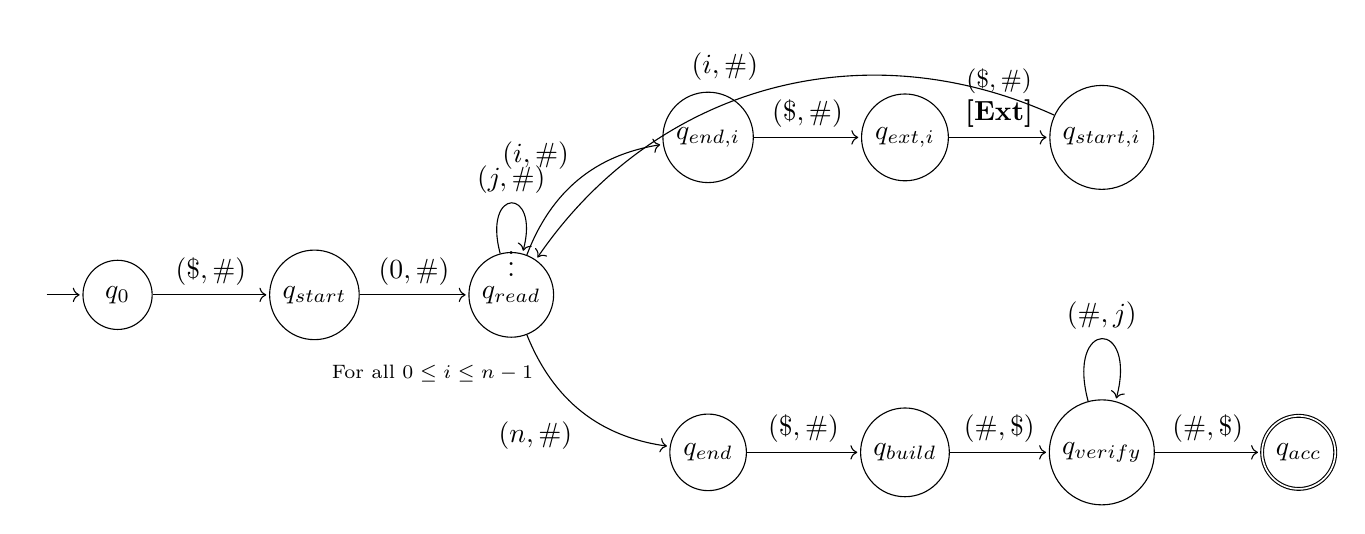
\begin{tikzpicture}[shorten >=1pt, node distance=2.5cm, on grid, auto, initial text=]
        
        %% NODES
        \node[state, initial] (q0) {$q_0$};
        \node[state] (qstart) [right=of q0] {$q_{start}$};
        \node[state] (qread) [right=of qstart] {$q_{read}$};
        
        % The generic "i" branch
        \node[state] (qendi) [above right=2cm and 2.5cm of qread] {$q_{end,i}$};
        \node[state] (qexti) [right=of qendi] {$q_{ext,i}$};
        \node[state] (qstarti) [right=of qexti] {$q_{start,i}$};
        
        % The exit to Part 2
        \node[state] (qend) [below right=2cm and 2.5cm of qread] {$q_{end}$};
        \node[state] (qbuild) [right=of qend] {$q_{build}$};
        \node[state] (qverify) [right=of qbuild] {$q_{verify}$};
        \node[state, accepting] (qacc) [right=of qverify] {$q_{acc}$};

        %% TRANSITIONS - PART 1 (x1 active)
        \path[->] 
            (q0) edge node {$(\$, \#)$} (qstart)
            (qstart) edge node {$(0, \#)$} (qread)
            (qread) edge [loop above] node {$(j, \#)$} (qread)
            
            % The "i" branch loop
            (qread) edge [bend left] node {$(i, \#)$} (qendi)
            (qendi) edge node {$(\$, \#)$} (qexti)
            (qexti) edge node [align=center] {\small $(\$, \#)$ \\ \textbf{[Ext]}} (qstarti)
            (qstarti) edge [bend right=40] node [swap] {$(i, \#)$} (qread);

        %% TRANSITIONS - PART 2 (x2 active)
        \path[->]
            (qread) edge [bend right] node [swap] {$(n, \#)$} (qend)
            (qend) edge node {$(\$, \#)$} (qbuild)
            
            (qbuild) edge node {$(\#, \$)$} (qverify)
            (qverify) edge [loop above] node {$(\#, j)$} (qverify)
            (qverify) edge node {$(\#, \$)$} (qacc);
            
        %% DECORATION (To show there are multiple branches)
        \node [above=0.5cm of qread] {$\vdots$};
        \node [font=\scriptsize, align=center] at (4, -1) {For all $0 \le i \le n-1$};
        
    \end{tikzpicture}
    \caption{Visual representation of the SQ-NFH. The upper loop represents the dynamic extension phase for $x_1$ (Part 1), verifying the chain links. The bottom path represents the validation phase for $x_2$ (Part 2), ensuring well-formedness.}
    \label{fig:sqnfh}
\end{figure}



\end{document}
